\chapter{Installation and operation manual}
\section{Introduction}
Due to the fact that Fantasy project is not an application that can be installed in a personal computer, but it is developed as a web application, it will have to be installed in a server.

\section{Previous requirements}
In order to install the application in the server, we need the Laravel framework, PHP, MySQL and Apache Server. Once those elements are installed, we will only have to launch the application from the directory of the project.

\section{Inventory of components}
The necesary components to launch Fantasy application would be:
\begin{itemize}
	\item Composer.
	\item Fantasy project with Laravel framework.
	\item PHP 7.3.
	\item MySQL.
	\item Apache Server.
	\item phpMyAdmin (optional).
\end{itemize}

\section{Installation procedures}
In order to install the components previously mentioned we shall follow the following steps:
\begin{itemize}
	\item Install PHP 7.3:
	\begin{itemize}
		\item \texttt{sudo apt-get -y install apt-transport-https lsb-release ca-certificates}
		\item \texttt{sudo wget -O /etc/apt/trusted.gpg.d/php.gpg https://packages.sury.org/php/\\apt.gpg}
		\item \texttt{sudo sh -c 'echo "deb https://packages.sury.org/php/ \$(lsb\_release -sc) main" > /etc/apt/sources.list.d/php.list'}
		\item \texttt{sudo apt-get update}
		\item \texttt{sudo apt-get install php7.3}
		\item \texttt{sudo apt install php7.3-cli php7.3-common php7.3-curl php7.3-mbstring \\php7.3-mysql php7.3-xml}
	\end{itemize}
	\item Install Apache Server:
	\begin{itemize}
		\item \texttt{sudo wget -O /etc/apt/trusted.gpg.d/php.gpg https://packages.sury.org/php/\\apt.gpg}
		\item \texttt{sudo sh -c 'echo "deb https://packages.sury.org/php/ \$(lsb\_release -sc) main" > /etc/apt/sources.list.d/php.list'}
		\item \texttt{sudo apt-get update}
		\item \texttt{sudo apt-get install apache2 -y}
		\item \texttt{sudo apt-get install libapache2-mod-php7.3}
	\end{itemize}
	\item Install composer:
	\begin{itemize}
		\item \texttt{php -r "copy('https://getcomposer.org/installer', 'composer-setup.php');"}
		\item \texttt{php -r "if (hash\_file('sha384', 'composer-setup.php') ===\\ '48e3236262b34d30969dca3c37281b3b4bbe3221bda826ac6a9a62d6444cdb0dcd06156\\98a5cbe587c3f0fe57a54d8f5') { echo 'Installer verified'; } else { echo\\ 'Installer corrupt'; unlink('composer-setup.php'); } echo PHP\_EOL;"}
		\item \texttt{sudo php composer-setup.php --install-dir=/usr/local/bin --filename=composer}
		\item \texttt{php -r "unlink('composer-setup.php');"}
	\end{itemize}
	\item Enable mod\_rewrite for Apache:
	\begin{itemize}
		\item \texttt{sudo a2enmod rewrite}
		\item \texttt{sudo service apache2 restart}
		\item \texttt{sudo apachectl -t -D DUMP\_MODULES | grep rewrite}
	\end{itemize}
	\item Download the Fantasy project folder in \texttt{/var/www/html/}.
	\item Unzip the file.
	\item Change pemissions with: \texttt{sudo chmod 777 -R Proyecto/}.
	\item Create an user with root access in MySQL.
	\item Create the fantasy database called ``fantasy''.
	\begin{itemize}
		\item \texttt{sudo mysql -u root -p}
		\newpage
		\item \texttt{create database fantasy;}
		\item \texttt{exit;}
	\end{itemize}
	\item Configure .env file:
	\begin{itemize}
		\item Rename \texttt{.env.example} file as \texttt{.env}
		\item Open \texttt{/var/www/html/Proyecto/.env} file.
%		\newpage
		\begin{figure}[h]
			\centering
			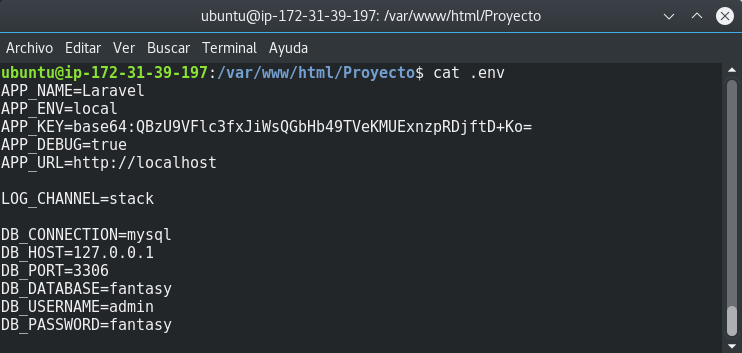
\includegraphics[scale=0.5]{Epilogue/env.png}
			\caption{.env file}
			\label{env file}
		\end{figure}
		APP\_NAME=Laravel\\
		APP\_ENV=local\\
		APP\_KEY= Generate with \texttt{sudo php artisan key:generate}\\
		APP\_DEBUG=true\\
		APP\_URL=http://localhost\\
		
		LOG\_CHANNEL=stack\\
		
		DB\_CONNECTION=mysql\\
		DB\_HOST=127.0.0.1\\
		DB\_PORT=3306\\
		DB\_DATABASE=fantasy\\
		DB\_USERNAME=admin (or root)\\
		DB\_PASSWORD=fantasy (password for admin/root)
	\end{itemize}
	\item \texttt{sudo php artisan migrate:fresh}
	\item Set up an Apache virtual host for your Laravel project:
	\begin{itemize}
		\item \texttt{sudo cp /etc/apache2/sites-available/000-default.conf /etc/apache2/sites-available/laravel.conf}
		\item \texttt{sudo nano /etc/apache2/sites-available/laravel\_project.conf}
		\item Modify the laravel\_project.conf contents so that they look like this:\\
		\texttt{<VirtualHost *:80>\\
			ServerName 54.162.132.90 (IP address of server)\\
			ServerAdmin alejandro.caraballogarcia@alum.uca.es\\
			DocumentRoot /var/www/html/Proyecto/public\\
			<Directory /var/www/html/Proyecto>\\
			AllowOverride All\\
			</Directory>\\
			ErrorLog \${APACHE\_LOG\_DIR}/error.log\\
			CustomLog \${APACHE\_LOG\_DIR}/access.log combined\\
			</VirtualHost>}
	\end{itemize}
	\item Enable new virtual host with \texttt{sudo a2ensite laravel\_project.conf}.
	\item \texttt{sudo awenmod rewrite}.
	\item Disable the default host with \texttt{sudo a2dissite 000-default.conf}.
	\item Restart Apache Server with \texttt{sudo services apache2 restart}.
	
\end{itemize}
\Nota
For more information, watch this \href{https://phpraxis.wordpress.com/2016/08/02/steps-for-configuring-laravel-on-apache-http-server/}{tutorial}.

\section{Implantation tests}
The implementation tests have been tested personally by the Fantasy team, verifying the possible configurations that could lead to an error, and they have been resolved mostly.

Those tests have been made in the Fantasy team's laptops and in a virtual machine EC2 from Amazon AWS.